\documentclass[12pt]{article}
\usepackage[utf8]{inputenc}
\usepackage[T2A]{fontenc}
\usepackage[russian]{babel}
\usepackage{amsmath}
\usepackage{amssymb}
\usepackage{dsfont}
\usepackage[dvipsnames]{xcolor}
\usepackage{setspace}
\usepackage{multirow}
\usepackage[a4paper, outer=1.5cm, inner=1.5cm, top=1cm, bottom=1cm]{geometry}
\usepackage{graphicx}
\usepackage{skull}
\usepackage{wasysym}
\usepackage{float}
\graphicspath{{.images/}}
\usepackage{hyperref}
\hypersetup{colorlinks=true, linkcolor=blue, filecolor=magenta, urlcolor=cyan}
\usepackage[firstpage]{draftwatermark}
\SetWatermarkText{
    $\qquad\qquad\qquad\qquad\qquad$\parbox{7cm}{\begin{center}
    
\includegraphics[width = 0.08\textwidth]{lion-logo.png}\bigskip\\~\bigskip\\~\vspace{-24mm}\\~\end{center}}
}
\SetWatermarkAngle{0}
\SetWatermarkScale{1.5}
\usepackage{etoolbox}

\newtoggle{ifsolved}
\newtoggle{needhelp}
\newcounter{num}
\setcounter{num}{1}

\newcommand{\newnum}{\par\textbf{\textnumero\arabic{num}}\stepcounter{num}}
\newcommand{\sol}{\vspace{3mm}\par\textbf{Решение: }}
\newcommand{\ans}{\vspace{3mm}\par\textbf{Ответ: }}
\newcommand{\hint}{\vspace{3mm}\par\textbf{Подсказка: }}
\newcommand{\mode}[1]{
\ifstrequal{#1}{0}{\togglefalse{ifsolved}\togglefalse{needhelp}}{\ifstrequal{#1}{1}{\togglefalse{ifsolved}\toggletrue{needhelp}}{\ifstrequal{#1}{2}{\toggletrue{ifsolved}\togglefalse{needhelp}}{\toggletrue{ifsolved}\toggletrue{needhelp}}}}} %if 0 - if 1 - if 2 - else
%\newenvironment{problem}[8]{%#1, #2, #3
%\parbox{\linewidth}{\vspace{4mm}\ifstrequal{#4}{(лёгкая)}{\newnum\textbf{.}}{\newnum\textbf{*.} } \\ #5}
%\iftoggle{ifsolved}{\sol #6}{}
%\iftoggle{ifsolved}{\ans #7}{}
%\iftoggle{needhelp}{\hint #8}{}}

\newenvironment{problem}[8]{%#1, #2, #3
\parbox{\linewidth}{\vspace{5mm}\ifstrequal{#4}{(лёгкая)}{\newnum\textbf{.}}{\newnum\textbf{*.} } \\ #5}
\iftoggle{ifsolved}{\sol #6}{}

\iftoggle{ifsolved}{\parbox{\linewidth}{\ans #7}}{}
\iftoggle{needhelp}{\parbox{\linewidth}{\hint #8}}{}}

\newenvironment{mylist} %custom list
{ \begin{itemize}
    \setlength{\itemsep}{0pt}
    \setlength{\parskip}{0pt}
    \setlength{\parsep}{0pt}     }
{ \end{itemize}                  }

\newenvironment{homeass}[1]{\vspace*{-1.5cm}
\iftoggle{ifsolved}{
    \section*{\center{Решение домашнего задания к #1.}}
}{
    \section*{\center{\textcolor{Sepia}{Домашнее задание к #1}}}
} \vspace{7mm}\large}

\parindent=0pt
\pagestyle{empty}
%$\!$[\arabic{class}.\arabic{num}]
%\ifnumcomp{\value{counter}}{>}{1}{true}{false}
%\definecolor{Gray}{gray}{0.9}
%\definecolor{mypink}{RGB}{219, 48, 122}
%\newcolumntype{g}{>{\columncolor{Gray}}p{2.8cm}}

\begin{document}
\large
\mode{7}
%0 for problems without hints
%1 for problems + hints
%2 for problems + solutions + answers
%else: show all

{\centering\section*{СПИСОК ЗАДАЧ}}

{\centering\subsection*{\smallskip\\\textcolor{green}{\textbf{Полезные вещи, которые можно и нужно копипастить:}}}}

\subsection*{\textcolor{Emerald}{\textbf{Полезные шпаргалки по LaTeXу:}}}

\textbf{Пример вставки рисунка:}

\begin{minipage}{\linewidth}
    \begin{minipage}{0.54\linewidth}
    см. рисунок справа\\
    Текст к собственно пикче, примерно всегда это либо развёрнутое описание, либо большая часть решения задачи --- стремимся экономить пространство, если это можно сделать.
    \end{minipage}
    \hspace{0.05\linewidth}
    \begin{minipage}{0.4\linewidth}
    \begin{figure}[H] 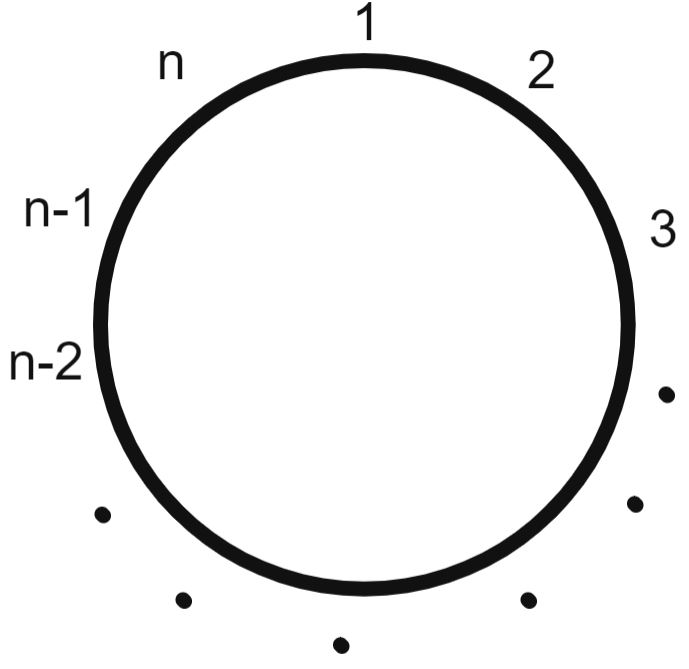
\includegraphics[width=\linewidth]{sol3} %тут поменять имя пикчи
    \end{figure}
    \end{minipage}
\end{minipage}

\textbf{Дефолтные математические знаки и символы:}\\
$\geqslant$,
$\leqslant$,
$a^{b}$,
$x_{i}$,
$\sqrt{a}$,
$\frac{a}{b}$,
$\displaystyle \frac{a}{b}$,
$\cdot$
$\;\Rightarrow\;$,
$\;\Leftrightarrow\;$,
$1{,}2$.
О промежутках:
$a\!b$,
$a\,b$,
$a\:b$,
$a\;b$,
$a\quad b$.

\textbf{Стандартные система и совокупность уравнений / неравенств:}\\
$\left\{
\begin{aligned}
f(x) &= 0 \\
g(x) &= 1
\end{aligned}\right.$

$\left[\begin{aligned}
&\left\{\begin{aligned}
f(x) &\geqslant a \\
g(x) &= b
\end{aligned}\right.\\
&\left\{\begin{aligned}
f(x) &< a \\
g(x) &= -b
\end{aligned}\right.
\end{aligned}\right.$

\subsection*{\textcolor{Emerald}{\textbf{Не математическое, но полезное:}}}
% комментарий в любом месте документа, который нигде не будет видно. Можно использовать для написания заметок-вопросов по задачам
\textbf{Пример таблицы:}

\begin{tabular}{|c|c|c|}
\hline
    $a$ & $b$ & текст
\\\hline
    $c$ & $d$ & мораль
\\\hline
\end{tabular}\\

\textbf{Отступы:} между\smallskip\\ строками\medskip\\ \textbf{Тире} --- это три дефиса.\\
\textbf{Списки:}
\begin{mylist}
\item [$\bullet$] это был пункт а
\item [2)] а это уже пункт номер 2 с изменённым заголовком
\end{mylist}

\subsection*{\textcolor{Emerald}{\textbf{Всё, неупомянутое выше (или если просто что-то не так):}}}
\begin{mylist}
\item [$\bullet$] Решение отдельных вопросов касательно ТеХа нужно искать в \href{https://www.mccme.ru/free-books/llang/newllang.pdf}{Львовском}.

\item [$\bullet$] Найти произвольный символ, который нужен, можно в \href{http://detexify.kirelabs.org/classify.html}{Detexify}.

\item [$\bullet$] Если возникли сомнения при решении, ответ практически ко всем задачам можно проверить с помощью \href{https://www.wolframalpha.com/}{WolframAlpha}.

\item [$\bullet$] Если в задаче нужно создать картинку, то лучше пока отложить эту задачу. Все графики планируется централизованно нарисовать (или перерисовать) в геогебре.

\item [\textcolor{brown}{\textbf{!!}}] Важно ставить \textcolor{red}{\textbf{$\spadesuit$}}
(или просто red) в тело задачи в случае серьёзных вопросов к решению и какой-то вопиющей лажи.

\item [\textcolor{brown}{\textbf{!!}}] Важно ставить \textcolor{olive}{\textbf{$\spadesuit$}}
(или просто olive) в тело задачи в случае не самого удачного текста и кривых отступов.
\end{mylist}

\subsection*{\textcolor{Violet}{\textbf{Комментарии:}}}% а также невидимые комментарии - так можно оставлять заметки-вопросы прямо в задаче, чтобы потом было понятно, в чём вопрос.
\begin{mylist}
\item [$\skull$] Переставлять задачи местами --- очень плохая идея.

\item [$\smiley$] При двойном клике по тексту pdf справа происходит автоматический переход к этому месту в латех-коде, а для обратного перехода можно нажать стрелку вправо (висит сверху между pdf и латех-кодом).

\item [$\smiley$] Если есть размышления, дописывать red/olive к задаче или не дописывать, то лучше всё-таки дописать.

\item [$\skull$] Самое плохое, что можно сделать --- написать в любое поле из трёх (НаписанноеРешение/ВерныйОтвет/Подсказка) только половину того, что надо, никак это не отметить, и потом пойти дальше.\\ Нужно в этот момент писать red/olive в случайном месте задачи, чтобы потом вычислить это с помощью Ctrl+F по всему документу (и это то, что потом будет делаться долго и тщательно)
\end{mylist}

\newpage
\setcounter{num}{100}

\hypertarget{6.4}{{\centering\section*{\bigskip\\\textcolor{Blue}{\hyperlink{start2}{\textcolor{Blue}{6.4}} Десятичные дроби и проценты.}\vspace{-5mm}}}}

\begin{problem}{Десятичная запись дробных чисел. Проценты.}{6.4.1}{6S}{(лёгкая)}
{Восстанови запись, где буква Й отлична от нуля: $\quad$ Х : О = К,КЕЙ.\\ Одинаковые буквы означают одинаковые цифры, разные буквы~--- разные цифры.

}
{НаписанноеРешение}
{ВерныйОтвет}{Подсказка}
\end{problem}

\begin{problem}{Десятичная запись дробных чисел. Проценты.}{6.4.1}{6K}{(лёгкая)}
{$\displaystyle\frac{1}{2} = 0{,}5,\; \frac{1}{4} = 0{,}25$. А чему равны $\displaystyle\frac{1}{8}$ и $\,\displaystyle\frac{1}{6}$? $\;$ А $\,\displaystyle\frac{1}{7}$?}
{НаписанноеРешение}
{ВерныйОтвет}{Подсказка}
\end{problem}

\begin{problem}{Десятичная запись дробных чисел. Проценты.}{6.4.1}{6S}{*}
{В классе 35 учеников, причём число мальчиков составляет 75\% от числа девочек. Сколько мальчиков в этом классе?}
{НаписанноеРешение}
{ВерныйОтвет}{Подсказка}
\end{problem}

\begin{problem}{Сравнение, сложение и вычитание десятичных дробей.}{6.4.2}{6S}{(лёгкая)}
{В числе $0{,}528047169$ вычеркни 4 знака после запятой, чтобы получилось:\\ 1) наибольшее число $\qquad$ 2) наименьшее число}
{НаписанноеРешение}
{ВерныйОтвет}{Подсказка}
\end{problem}

\begin{problem}{Сравнение, сложение и вычитание десятичных дробей.}{6.4.2}{6S}{(лёгкая)}
{В числе $1037{,}584629$ вычеркни 3 цифры так, чтобы оставшиеся цифры в том же порядке составили:\\ 1) наибольшее число $\qquad$ 2) наименьшее число}
{НаписанноеРешение}
{ВерныйОтвет}{Подсказка}
\end{problem}

\begin{problem}{Сравнение, сложение и вычитание десятичных дробей.}{6.4.2}{6S}{(лёгкая)}
{Найти сумму $\;0{,}01 + 0{,}02 + 0{,}03 + \ldots + 0{,}98 + 0{,}99$.}
{НаписанноеРешение}
{ВерныйОтвет}{Подсказка}
\end{problem}

\begin{problem}{Сравнение, сложение и вычитание десятичных дробей.}{6.4.2}{6S}{(лёгкая)}
{Пешеход прошёл 70\% намеченного пути и установил, что ему осталось пройти на $8{,}6$ км меньше пройденного. Сколько всего километров должен был пройти пешеход?}
{НаписанноеРешение}
{ВерныйОтвет}{Подсказка}
\end{problem}

\begin{problem}{Сравнение, сложение и вычитание десятичных дробей.}{6.4.2}{6S}{*}
{20\% числа $x$ больше 20. Сравнить число $x$ и 100.}
{НаписанноеРешение}
{ВерныйОтвет}{Подсказка}
\end{problem}

\begin{problem}{Умножение десятичных дробей и нахождение части числа.}{6.4.3}{6S}{(лёгкая)}
{Какой цифрой оканчивается сумма $\;\displaystyle 1{,}7 \cdot 5 \cdot 2{,}9 \cdot 2 + 3{,}1 \cdot 25 \cdot 6{,}3 \cdot 4$?}
{НаписанноеРешение}
{ВерныйОтвет}{Подсказка}
\end{problem}

\begin{problem}{Умножение десятичных дробей и нахождение части числа.}{6.4.3}{6S}{(лёгкая)}
{К какому числу надо прибавить $27{,}31$, чтобы получить число в $3{,}5$ раза больше, чем $18{,}4$?}
{НаписанноеРешение}
{ВерныйОтвет}{Подсказка}
\end{problem}

\begin{problem}{Умножение десятичных дробей и нахождение части числа.}{6.4.3}{6S}{(лёгкая)}
{Если к неизвестному числу прибавить $2{,}5$, сумму умножить на 4 и произведение разделить на $0{,}5$, то получится 50. Найти это число.}
{НаписанноеРешение}
{ВерныйОтвет}{Подсказка}
\end{problem}

\begin{problem}{Умножение десятичных дробей и нахождение части числа.}{6.4.3}{6S}{(не лёгкая)}
{Масса куриного яйца равна 80 г.\\ Белок составляет 55\% всей массы, а желток~--- 75\% массы белка.\\ Узнай, какова масса скорлупы (кроме белка и желтка больше ничего нет).}
{Так как белок составляет 55\% всей массы, выясним, какую массу имеют 5\% яйца: $5\% = \frac{5}{100} = \frac{1}{20}$, поэтому масса равна $80 \cdot \frac{1}{20} = 4$ г.\\ Масса белка в 11 раз больше, чем 55\%, и потому равна $4\cdot11 = 44$ г. Желток составляет $75\% = \frac34$ от этого, а значит, имеет массу $44 \cdot \frac34 = 11 \cdot 3 = 33$ г.\\ Вместе желток и белок весят $44 + 33 = 77$ г. Так как кроме белка, желтка и скорлупы в яйце больше ничего нет, масса скорлупы равна $80 - 77 = 3$ г.}
{Масса скорлупы равна 3 г.}{Найди $5\%$ массы яйца. Какова масса белка? Желтка?}
\end{problem}

\begin{problem}{Умножение десятичных дробей и нахождение части числа.}{6.4.3}{6S}{(не лёгкая)}
{Катя купила чайник за 180 рублей и 6 чашек по цене 120 рублей/чашка. Через неделю магазин повысил цену чашки на 10\%, а цену чайника снизил на 15\%. \\ Увеличилась или уменьшилась при этом стоимость всей покупки и на сколько?}
{10\% стоимости чашки, или $\frac{1}{10}$ --- 12 рублей. 15\% стоимости чайника --- $18 + 9 = 27$ рублей. Таким образом, теперь чашка стоит $120 + 12 = 132$ рубля, а чайник --- $180 - 27 = 153$ рубля. Вычислим общую сумму покупки сейчас и неделю назад: $180 + 6 \cdot 120 = 180 + 720 = 900$ рублей (общая стоимость неделю назад), $153 + 6 \cdot 132 = 153 + 792 = 945$ рублей (общая стоимость покупки теперь).\\
Таким образом, за эту неделю стоимость покупки увеличилась, она возросла на 45 рублей (или на 5\% общей стоимости).}
{Стоимость всей покупки увеличилась на 45 рублей.}{Какой стала цена каждой чашки и чайника через неделю?}
\end{problem}

\begin{problem}{Умножение десятичных дробей и нахождение части числа.}{6.4.3}{6K}{(лёгкая)}
{На день рождения, $7$-классники пошли в аквапарк, за который они ожидали заплатить $18380$ рублей. Однако, оказалось, что в день рождения действует скидка в $15\%$. Сколько пришлось заплатить?}
{Поскольку в итоге в аквапарке действовала скидка, найдём 85\% от общей стоимости: $18380 \cdot 0{,}15 = 1838 \cdot 1{,}5 = 1838 + 919 = 2757$ рублей --- величина скидки. Следовательно, всего пришлось заплатить $18380 - 2757 = 15623$ рубля.}
{Всего пришлось заплатить 15623 рубля.}{Какова величина скидки?}
\end{problem}

\begin{problem}{Умножение десятичных дробей и нахождение части числа.}{6.4.3}{6K}{(лёгкая)}
{Зарплату токарю сначала повысили на $10\%$, а затем через год повысили ещё на $20\%$. На сколько процентов повысилась зарплата токаря по сравнению с первоначальной?}
{НаписанноеРешение}
{ВерныйОтвет}{Подсказка}
\end{problem}

\begin{problem}{Умножение десятичных дробей и нахождение части числа.}{6.4.3}{6K}{(лёгкая)}
{В городе N сначала снесли $10\%$ всех детских площадок, пообещав потом построить новые, а в следующем году выполнили обещание, увеличив количество детских площадок на $25\%$ (по сравнению с тем числом, что осталось после сноса).\\ На сколько процентов в результате изменилось общее число площадок в городе, если до сноса было всего $400$ детских площадок?}
{Было снесено $400 \cdot \frac{1}{10} = 40$ детских площадок. После этого осталось $400 - 40 = 360$ площадок. Одна четверть от этого количества --- это $360 \cdot \frac{1}{4} = 90$, поэтому после увеличения количества площадок на 25\%, всего будет $360 + 90 = 450$ детских площадок. Таким образом, в результате этих действий общее количество детских площадок в городе N увеличилось на 50 штук.\\ Это составляет $\frac{50}{400} = \frac18 = 12{,}5\%$ от числа площадок до сноса.}
{Общее число площадок в городе возросло на 12{,}5\%.}{Сколько площадок осталось в городе N после сноса?}
\end{problem}

\begin{problem}{Умножение десятичных дробей и нахождение части числа.}{6.4.3}{6K}{(лёгкая)}
{У эльфов в бочонках было $290$ галлонов вина. После побега гномов, $18\%$ вина было утрачено. Сколько галлонов вина осталось у эльфов?}
{НаписанноеРешение}
{ВерныйОтвет}{Подсказка}
\end{problem}

\begin{problem}{Умножение десятичных дробей и нахождение части числа.}{6.4.3}{6K}{*}
{Все плюшевые игрушки производятся на трёх фабриках: половина игрушек на первой фабрике, треть на второй, и $\frac{1}{6}$~--- на третьей. На второй фабрике что-то случилось, и в результате три четверти всех игрушек оттуда приехали испачканными. Сколько процентов от ВСЕХ игрушек остались не испачканными?}
{НаписанноеРешение}
{ВерныйОтвет}{Подсказка}
\end{problem}

\begin{problem}{Умножение десятичных дробей и нахождение части числа.}{6.4.3}{6K}{(лёгкая)}
{В супермаркете проводится акция. Коробка конфет некоторого вида стоит 360 рублей. При покупке двух таких коробок на вторую коробку предоставляется скидка в размере 45\%. Сколько рублей придётся заплатить за покупку двух коробок конфет в период действия акции?}
{НаписанноеРешение}
{ВерныйОтвет}{Подсказка}
\end{problem}

\begin{problem}{Умножение десятичных дробей и нахождение части числа.}{6.4.3}{6K}{(лёгкая)}
{Бутылку общим объёмом $600$ миллилитров, заполненную на $25\%$, наполнили ещё на треть от общего объёма. Какой объём бутылки остался пустым?}
{НаписанноеРешение}
{ВерныйОтвет}{Подсказка}
\end{problem}

\begin{problem}{Умножение десятичных дробей и нахождение части числа.}{6.4.3}{6S}{(лёгкая)}
{Сапоги стоили 300 р. Цена на них последовательно понижалась два раза на 10\%. \\ Какой стала цена сапог после второго понижения?}
{НаписанноеРешение}
{ВерныйОтвет}{Подсказка}
\end{problem}

\begin{problem}{Умножение десятичных дробей и нахождение части числа.}{6.4.3}{6S}{(лёгкая)}
{Свитер стоил 250 р. Цена на него последовательно повышалась два раза на 10\%. \\ Какой стала цена свитера после второго повышения?}
{НаписанноеРешение}
{ВерныйОтвет}{Подсказка}
\end{problem}

\begin{problem}{Умножение десятичных дробей и нахождение части числа.}{6.4.3}{6K red}{(лёгкая)}
{Вычислить значение: \hfill 1) $0{,}8 \cdot 1{,}2$; \hfill 2) $0{,}8 \cdot 1{,}25$.\hspace*{2cm}\\
Сделай выводы.}
{НаписанноеРешение}
{ВерныйОтвет}{Подсказка}
\end{problem}

\begin{problem}{Умножение десятичных дробей и нахождение части числа.}{6.4.3}{9I}{(лёгкая)}
{Цену на некоторый товар сначала снизили на 10\%, затем снизили ещё на четверть, а через некоторое время~--- повысили на 20\%. На сколько процентов первоначальная цена товара выше конечной?}
{НаписанноеРешение}
{ВерныйОтвет}{Подсказка}
\end{problem}

\begin{problem}{Умножение десятичных дробей и нахождение части числа.}{6.4.3}{6K}{(лёгкая)}
{Магазин повысил цены на $20\%$, а затем понизил новую цену на $20\%$.\\ На сколько процентов изменилась цена? В чём подвох?}
{НаписанноеРешение}
{ВерныйОтвет}{Подсказка}
\end{problem}

\begin{problem}{Умножение десятичных дробей и нахождение части числа.}{6.4.3}{6K}{(лёгкая)}
{Гэндальф имел рост 1 м 85 см. Рост гнома Гимли составляет $40\%$ от роста Гэндальфа. Найти рост Гимли.}
{НаписанноеРешение}
{ВерныйОтвет}{Подсказка}
\end{problem}

\begin{problem}{Умножение десятичных дробей и нахождение части числа.}{6.4.3}{6K}{(лёгкая)}
{Магазин продал одному покупателю $25\%$ имевшегося в куске полотна, второму покупателю~--- $30\%$ остатка, а третьему покупателю~--- $40\%$ нового остатка. Сколько процентов полотна осталось непроданным?}
{НаписанноеРешение}
{ВерныйОтвет}{Подсказка}
\end{problem}

\begin{problem}{Умножение десятичных дробей и нахождение части числа.}{6.4.3}{6S}{(лёгкая)}
{В одном магазине молоко подешевело на 40\%, а в другом~--- сначала на 20\%, а затем ещё на 25\%. Где молоко стало стоить дешевле? В начале цена на молоко в обоих магазинах была одна и та же.}
{НаписанноеРешение}
{ВерныйОтвет}{Подсказка}
\end{problem}

\begin{problem}{Умножение десятичных дробей и нахождение части числа.}{6.4.3}{6S}{(лёгкая)}
{Каждую сторону квадрата увеличили на 20\%.\\ На сколько процентов увеличилась площадь квадрата?}
{НаписанноеРешение}
{ВерныйОтвет}{Подсказка}
\end{problem}

\begin{problem}{Умножение десятичных дробей и нахождение части числа.}{6.4.3}{6S}{(лёгкая)}
{На сколько процентов увеличится площадь квадрата, если его периметр увеличить на 10\%?}
{НаписанноеРешение}
{ВерныйОтвет}{Подсказка}
\end{problem}

\begin{problem}{Умножение десятичных дробей и нахождение части числа.}{6.4.3}{6S}{(лёгкая)}
{Две противоположные стороны прямоугольника увеличили на 10\%, а две другие укоротили на 10\%. Как изменилась площадь прямоугольника?}
{НаписанноеРешение}
{ВерныйОтвет}{Подсказка}
\end{problem}

\begin{problem}{Умножение десятичных дробей и нахождение части числа.}{6.4.3}{6S}{(лёгкая)}
{На сколько процентов увеличится объём куба, если каждое его ребро увеличить на 10\%?}
{НаписанноеРешение}
{ВерныйОтвет}{Подсказка}
\end{problem}

\begin{problem}{Умножение десятичных дробей и нахождение части числа.}{6.4.3}{6S}{(лёгкая)}
{На сколько процентов уменьшится объём куба, если длину каждого его ребра уменьшить на 20\%?}
{НаписанноеРешение}
{ВерныйОтвет}{Подсказка}
\end{problem}

\begin{problem}{Деление десятичных дробей и нахождение числа по его части.}{6.4.4}{6S}{(лёгкая)}
{Найди такое число, чтобы, увеличив его в 100 раз и прибавив к произведению $3{,}2$, получить $256{,}7$.}
{НаписанноеРешение}
{ВерныйОтвет}{Подсказка}
\end{problem}

\begin{problem}{Деление десятичных дробей и нахождение числа по его части.}{6.4.4}{6S}{(лёгкая)}
{Если из задуманного числа вычесть $1{,}05$, разность умножить на $0{,}8$, к произведению прибавить $2{,}84$, полученную сумму разделить на $0{,}01$, то получится 700. Какое число было задумано?}
{Все упомянутые в задаче действия можно записать в строчку: если было задумано число $n$, то $((n - 1{,}05) \cdot 0{,}8 + 2{,}84) : 0{,}01 = 700$. Это значит, что:\\
$(n - 1{,}05) \cdot 0{,}8 + 2{,}84 = 700 \cdot 0{,}01 = 7 \;\Rightarrow\;$\\
$(n - 1{,}05) \cdot 0{,}8 = 7 - 2{,}84 = 4{,}16 \;\Rightarrow\; n - 1{,}05 = 4{,}16 : 0{,}8 = 416 : 80 = 5{,}2 \;\Rightarrow\;$\\
$n - 1{,}05 = 5{,}2 \;\Rightarrow\; n = 5{,}2 + 1{,}05 = 6{,}25$.}
{Было задумано число $6{,}25$.}{Выполни все арифметические действия в обратном порядке.}
\end{problem}

\begin{problem}{Деление десятичных дробей и нахождение числа по его части.}{6.4.4}{6S}{(лёгкая)}
{Если к задуманному числу прибавить $0{,}43$ его, а затем от полученного результата отнять $0{,}58$ задуманного числа и ещё $4{,}04$, то получим $30{,}3$.\\ Найти задуманное число.}
{Допустим, задуманное число~--- $A$.\\ Тогда, следуя условию, получаем уравнение $A + 0{,}43A - 0{,}58A - 4{,}04 = 30{,}3$. $\;A + 0{,}43A - 0{,}58A = 1{,}43A - 0{,}58A = 0{,}85A$. Отсюда $\,0{,}85A - 4{,}04 = 30{,}3 \;\Rightarrow\; 0{,}85A = 30{,}3 + 4{,}04 = 34{,}34$. Таким образом, $0{,}85A = 34{,}34$. Как мы знаем, если $ab = c$, то $b = \frac ca$. Поэтому делим обе части уравнения на $0{,}85$ и находим $A$:\smallskip\\
$A = 34{,}34 : 0{,}85 = \frac{34{,}34}{0{,}85} = \frac{3434}{85} = \frac{\textcolor{blue}{17}\cdot 202}{\textcolor{blue}{17}\cdot 5} = \frac{202}{5} = 40{,}4$.}
{Было задумано число $40{,}4$.}{Пусть было задумано некоторое число $A$.\\ Какое уравнение мы тогда получаем?}
\end{problem}

\begin{problem}{Деление десятичных дробей и нахождение числа по его части.}{6.4.4}{6S}{(лёгкая)}
{Сколько килограммов белых грибов надо собрать для получения 1 кг сушёных, если при подготовке к сушке остаётся $0{,}5$ веса собранных грибов, а при сушке остаётся $0{,}1$ веса обработанных грибов?}
{НаписанноеРешение}
{ВерныйОтвет}{Подсказка}
\end{problem}

\begin{problem}{Деление десятичных дробей и нахождение числа по его части.}{6.4.4}{6S}{(лёгкая)}
{Запас муки был распределён между тремя пекарнями. Первая получила $0{,}4$ всего запаса, вторая~--- $0{,}4$ остатка, а третья пекарня получила муки на $1{,}6$ т меньше, чем первая. Сколько всего муки было распределено?}
{НаписанноеРешение}
{ВерныйОтвет}{Подсказка}
\end{problem}

\begin{problem}{Деление десятичных дробей и нахождение числа по его части.}{6.4.4}{6K}{(лёгкая)}
{За неделю книжный магазин продал $1053$ книги, что составило лишь $54\%$ от книг, привезённых в магазин в этом месяце.\\ Сколько книг привезли в магазин в этом месяце?}
{НаписанноеРешение}
{ВерныйОтвет}{Подсказка}
\end{problem}

\begin{problem}{Деление десятичных дробей и нахождение числа по его части.}{6.4.4}{6K}{(лёгкая)}
{За месяц химик потратил $36$ кг реагентов, что составило лишь $16\%$ от количества реагентов, которые находились в его лаборатории.\\ Сколько килограмм реагентов находилось в лаборатории в начале месяца?}
{Если 36 килограмм реагентов --- это только $16\%$ от количества реагентов в лаборатории, то 4\% в 4 раза меньше этого, то есть это 9 килограмм.\\ Тогда в начале месяца реагентов в лаборатории было в 25 раз больше (так как $4\% = \frac{1}{25}$), а значит, их всего было $9 \cdot 25 = 225$ кг.}
{Всего в лаборатории в начале месяца было 225 кг реагентов.}{Сколько килограмм реагентов составляет 4\% от количества реагентов, которые были в лаборатории в начале месяца?}
\end{problem}

\begin{problem}{Деление десятичных дробей и нахождение числа по его части.}{6.4.4}{6K}{(лёгкая)}
{Зарядка для телефона со скидкой в 25\% стоит 120 рублей.\\ Сколько она стоит без скидки?}
{Поскольку 120 рублей --- стоимость со скидкой, эта цена равна 75\% от начальной. Следовательно, 25\% цены --- в три раза меньше, или $120 : 3 = 40$ рублей. Следовательно, полная цена без скидки составляет 100\%, что в 4 раза больше. Поэтому без скидки зарядка стоит $40 \cdot 4 = 160$ рублей.}
{Стоимость зарядки без скидки составляет 160 рублей.}{Какую часть цены зарядки составляют 120 рублей?}
\end{problem}

\begin{problem}{Деление десятичных дробей и нахождение числа по его части.}{6.4.4}{6K}{(лёгкая)}
{За день овощной отдел магазина продал $750$ кг картофеля, что составило $15\%$ от всего количества картофеля, завезённого в магазин.\\ Сколько тонн картофеля завезли в магазин?}
{НаписанноеРешение}
{ВерныйОтвет}{Подсказка}
\end{problem}

\begin{problem}{Деление десятичных дробей и нахождение числа по его части.}{6.4.4}{6K}{(лёгкая)}
{Поезд метро в час пик за $5$ минут проехал $5$ километров, а поздно вечером за $4$ минуты он проехал только $3$ километра.\\ На сколько процентов уменьшилась скорость поезда к вечеру?}
{НаписанноеРешение}
{ВерныйОтвет}{Подсказка}
\end{problem}

\begin{problem}{Деление десятичных дробей и нахождение числа по его части.}{6.4.4}{6S}{(лёгкая)}
{Когда турист прошёл $0{,}35$ всего пути, до половины ему оставалось пройти всего лишь 6 км. Найти длину всего пути.}
{Поскольку 6 километров --- то, сколько туристу осталось пройти до половины, это разница между половиной и $0{,}35$.\\ Поэтому получается, что $6$ километров --- это $0{,}5 - 0{,}35 = 0{,}15$ всего пути.\\
Тогда втрое меньшая величина, 2 километра --- это $0{,}15 : 3 = 0{,}05 = \frac{1}{20}$ всего пути. Весь путь в 20 раз длиннее и поэтому имеет длину $2 \cdot 20 = 40$ км.}
{Длина всего пути составляет 40 км.}{Какую часть пути составляют упомянутые 6 км?}
\end{problem}

\begin{problem}{Деление десятичных дробей и нахождение числа по его части.}{6.4.4}{6S}{(лёгкая)}
{Железнодорожный билет со скидкой в 20\% стоит 100 р.\\ Сколько он стоит без скидки?}
{НаписанноеРешение}
{ВерныйОтвет}{Подсказка}
\end{problem}

\begin{problem}{Деление десятичных дробей и нахождение числа по его части.}{6.4.4}{6S}{(лёгкая)}
{Альбом сейчас стоит 270р. Какова была стоимость альбома до снижения, если две недели назад цену снизили на 25\%, а затем ещё на 20\% от новой стоимости?}
{270 рублей --- цена после второго снижения стоимости, то есть это 80\% от какой-то промежуточной цены. В таком случае 20\% этой цены в 4 раза меньше, а именно $270 : 4 = 67{,}5$ р. Значит, до второго снижения цена составляла $270 + 67{,}5 = 337{,}5$ р. Это цена, которая получилась после снижения первоначальной цены на 25\%. Значит, она составляет 75\% первоначальной цены альбома.\\ Следовательно, 25\% начальной цены альбома втрое меньше: $337{,}5 : 3 = 112{,}5$. Значит, первоначальная цена альбома составляет $337{,}5 + 112{,}5 = 450$ рублей.}
{До снижения альбом стоил 450 рублей.}{Какая была цена альбома до последнего снижения цены на 20\%?}
\end{problem}

\begin{problem}{Деление десятичных дробей и нахождение числа по его части.}{6.4.4}{6S}{(лёгкая)}
{Фрукты при сушке теряют 82\% своего веса. \\Сколько надо взять свежих фруктов, чтобы получить 36 кг сушёных?}
{НаписанноеРешение}
{ВерныйОтвет}{Подсказка}
\end{problem}

\begin{problem}{Деление десятичных дробей и нахождение числа по его части.}{6.4.4}{6K}{(лёгкая)}
{В магазине идёт большая распродажа, и на все товары действует скидка $35\%$. Некто зашёл в магазин и купил себе палатку, стул-раскладушку, горные ботинки и набор батареек, заплатив всего $x$ рублей.\\ Сколько ему пришлось бы заплатить, если бы в этот день распродажи не было?}
{НаписанноеРешение}
{ВерныйОтвет}{Подсказка}
\end{problem}

\begin{problem}{Деление десятичных дробей и нахождение числа по его части.}{6.4.4}{6K}{*}
{Арктический заяц-беляк за $15$ секунд может пробежать $225$ метров, а лиса может пробежать $250$ метров за $18$ секунд. Кто из них быстрее и на сколько процентов?}
{Определим скорости обоих: скорость зайца равна $\frac{225}{15} = 15$ м/c, а скорость лисы равна $\frac{250}{18} = \frac{125}{9} = 13\frac89$ м/c. Таким образом, заяц быстрее, чем лиса.\smallskip\\ Выясним, на сколько он быстрее: $15 - 13\frac89 = \frac{10}{9}$ м/с --- это разница в их скоростях. Это составляет $\frac{10}{9} : \frac{125}{9} = \frac{10}{125} = \frac{2}{25} = 0{,}08$ от скорости лисы.\\ Следовательно, скорость зайца больше скорости лисы на 8\%.}
{Заяц-беляк бегает на 8\% быстрее лисы.}{Каковы скорости зайца и лисы?}
\end{problem}

\begin{problem}{Деление десятичных дробей и нахождение числа по его части.}{6.4.4}{6K}{(лёгкая)}
{За $9$ метров скатерти и $8{,}5$ метров ткани уплачено $5688$ рублей. Сколько стоила скатерть, а сколько~--- ткань, если $1$ метр скатерти на $25\%$ дороже $1$ метра ткани?

}
{НаписанноеРешение}
{ВерныйОтвет}{Подсказка}
\end{problem}

\begin{problem}{Деление десятичных дробей и нахождение числа по его части.}{6.4.4}{6K}{(лёгкая)}
{За неделю сладкоежка Василий съел $4212$ г сладкого, что составило лишь $52\%$ от запасов сладкого, которые были у него дома.\\ Сколько килограммов сладкого было у него дома в начале недели?}
{НаписанноеРешение}
{ВерныйОтвет}{Подсказка}
\end{problem}

\begin{problem}{Деление десятичных дробей и нахождение числа по его части.}{6.4.4}{6K}{(лёгкая)}
{За неделю отличник Петя решил $24$ задачи, что составило $32\%$ от количества задач, которые Петя планировал решить. Сколько всего было задач?}
{НаписанноеРешение}
{ВерныйОтвет}{Подсказка}
\end{problem}

\begin{problem}{Деление десятичных дробей и нахождение числа по его части.}{6.4.4}{6S}{(лёгкая)}
{Если увеличить длину прямоугольника на 25\%, то на сколько надо уменьшить его ширину, чтобы площадь не изменилась?}
{НаписанноеРешение}
{ВерныйОтвет}{Подсказка}
\end{problem}

\begin{problem}{Деление десятичных дробей и нахождение числа по его части.}{6.4.4}{6S}{(лёгкая)}
{Ширину прямоугольника увеличили на $3{,}6$ см, а длину уменьшили на 16\%. В результате площадь нового прямоугольника оказалась на 5\% больше площади прежнего. Найти ширину нового прямоугольника.}
{НаписанноеРешение}
{ВерныйОтвет}{Подсказка}
\end{problem}

\begin{problem}{Дробные выражения.}{6.4.5}{6K}{(лёгкая)}
{Чему равна разность $\;\displaystyle\frac{2}{0{,}5} - \frac{0{,}8}{6{,}4}$?}
{НаписанноеРешение}
{ВерныйОтвет}{Подсказка}
\end{problem}

\begin{problem}{Дробные выражения.}{6.4.5}{6K}{(лёгкая)}
{Чему равна сумма $\;\displaystyle\frac{2{,}5}{1{,}4} + \frac{2{,}3}{4{,}2}$?}
{Приведём дроби к общему знаменателю:\smallskip\\ $\displaystyle\frac{2{,}5}{1{,}4} + \frac{2{,}3}{4{,}2} = \frac{25}{14} + \frac{23}{42} = \frac{75}{42} + \frac{23}{42} = \frac{75 + 23}{42} = \frac{\textcolor{green}{98}}{\textcolor{green}{42}} = \frac{\textcolor{blue}{49}}{\textcolor{blue}{21}} = \frac{7}{3} = 2\frac13$.}
{$\;\displaystyle\frac{2{,}5}{1{,}4} + \frac{2{,}3}{4{,}2} = 2\frac13$.}{Можно домножить и числитель, и знаменатель дробей на 10...}
\end{problem}

\begin{problem}{Дробные выражения.}{6.4.5}{6K}{(лёгкая)}
{Чему равна разность $\;\displaystyle\frac{2{,}1}{0{,}7} - \frac{0{,}35}{1{,}05}$?}
{Домножим числители и знаменатели на 10 и 100:\smallskip\\
$\;\displaystyle\frac{2{,}1}{0{,}7} - \frac{0{,}35}{1{,}05} = \frac{\textcolor{orange}{21}}{\textcolor{orange}{7}} - \frac{\textcolor{violet}{35}}{\textcolor{violet}{105}} = 3 - \frac13 = 2\frac23$.}
{$\;\displaystyle\frac{2{,}1}{0{,}7} - \frac{0{,}35}{1{,}05} = 2\frac23$.}{Можно домножить и числитель, и знаменатель дробей на 10...}
\end{problem}

\begin{problem}{Дробные выражения.}{6.4.5}{6K}{(лёгкая)}
{Чему равна сумма $\;\displaystyle\frac{3}{0{,}8} + \frac{0{,}4}{1{,}6}$?}
{НаписанноеРешение}
{ВерныйОтвет}{Подсказка}
\end{problem}

\begin{problem}{Дробные выражения.}{6.4.5}{6K}{(лёгкая)}
{Чему равно выражение $\;\displaystyle 2 - \frac{\frac{1{,}5}{2{,}8}}{\frac{0{,}3}{0{,}42}}$?}
{Учтём, что $\frac{a}{b} = a : b$, тогда $\displaystyle 2 - \frac{\frac{1{,}5}{2{,}8}}{\frac{0{,}3}{0{,}42}} = 2 - \frac{1{,}5}{2{,}8} : \frac{0{,}3}{0{,}42} = 2 - \frac{1{,}5}{2{,}8} \cdot \frac{0{,}42}{0{,}3} =$ $\displaystyle 2 - \frac{\textcolor{orange}{15}}{\textcolor{violet}{28}} \cdot \frac{\textcolor{violet}{42}}{\textcolor{orange}{30}} = 2 - \frac{1\cdot\textcolor{Emerald}{6}}{4\cdot\textcolor{Emerald}{2}} = 2 - \frac{3}{4} = \frac54 = 1{,}25$.}
{$\:\displaystyle 2 - \frac{\frac{1{,}5}{2{,}8}}{\frac{0{,}3}{0{,}42}} = 1{,}25$.}{$\:\frac ab = a : b$, а делить дробь на дробь мы умеем.}
\end{problem}

\begin{problem}{Дробные выражения.}{6.4.5}{6K}{(лёгкая)}
{Найти значение выражения $\;8{,}4 : \left(\displaystyle \frac{1{,}6 \cdot 0{,}5}{1 - \frac{1}{9}} - \frac{2{,}1 + 16 \cdot 0{,}2}{(9{,}2 - 8{,}8) \cdot 17{,}5}\right) = {?}$\\ Ответ записать в виде десятичной дроби.}
{НаписанноеРешение}
{ВерныйОтвет}{Подсказка}
\end{problem}

\begin{problem}{Дробные выражения.}{6.4.5}{6K}{*}
{Вычислить: $\,\displaystyle 1\frac{18}{25} + 2\cdot\left(\frac{1}{20} + \frac{1}{100}\right) - 2\cdot \left(\frac{4}{3} - \frac{1}{4}\cdot\frac{1}{12}\right)\cdot 0{,}5 + 1{,}5\cdot1{,}5$ \\Ответ дать в виде десятичной дроби.}
{НаписанноеРешение}
{ВерныйОтвет}{Подсказка}
\end{problem}

\begin{problem}{Дробные выражения.}{6.4.5}{56}{(лёгкая)}
{Найти значение выражения: $\;\displaystyle \frac{\left(\left(40 \frac{7}{30} - 38 \frac{5}{12}\right) : 10{,}9 + \left(\frac{7}{8} - \frac{7}{30}\right) \cdot 1\frac{9}{11}\right) \cdot 4{,}2}{0{,}008}$}
{НаписанноеРешение}
{ВерныйОтвет}{Подсказка}
\end{problem}

\begin{problem}{Дробные выражения.}{6.4.5}{56}{(лёгкая)}
{Найти значение выражения: $\;\displaystyle 6{,}4 : \left(\frac{6 : \left(0{,}3 - 0{,}1\right)}{0{,}5 \cdot \left(1{,}6 + 0{,}4\right)} + \frac{3{,}6 : \left(4{,}3 - 2{,}5\right)}{\left(8{,}2 - 7{,}8\right) \cdot 2{,}5} \right)$.}
{Определим порядок действий: $\;6{,}4 \overset{\normalsize{\textcolor{Emerald}{10}}}{\mathstrut \!:} \left(\frac{6 \overset{\normalsize{\textcolor{Emerald}{2}}}{\mathstrut :} \left(0{,}3 \overset{\normalsize{\textcolor{Emerald}{1}}}{\mathstrut -} 0{,}1\right)}{0{,}5 \overset{\normalsize{\textcolor{Emerald}{4}}}{\mathstrut \cdot} \left(1{,}6 \overset{\normalsize{\textcolor{Emerald}{3}}}{\mathstrut +} 0{,}4\right)} \overset{\normalsize{\textcolor{Emerald}{9}}}{\mathstrut +} \frac{3{,}6 \overset{\normalsize{\textcolor{Emerald}{6}}}{\mathstrut :} \left(4{,}3 \overset{\normalsize{\textcolor{Emerald}{5}}}{\mathstrut -} 2{,}5\right)}{\left(8{,}2 \overset{\normalsize{\textcolor{Emerald}{7}}}{\mathstrut -} 7{,}8\right) \overset{\normalsize{\textcolor{Emerald}{8}}}{\mathstrut \cdot} 2{,}5} \right)$.\\
1) $0{,}3 - 0{,}1 = 0{,}2 = \frac15$.\smallskip\\
2) $6 : \frac15 = 6 \cdot 5 = 30$.\smallskip\\
3) $1{,}6 + 0{,}4 = 2$.\smallskip\\
4) $0{,}5 \cdot 2 = \frac12 \cdot 2 = 1$.\smallskip\\
5) $4{,}3 - 2{,}5 = 1{,}8$.\smallskip\\
6) $3{,}6 : 1{,}8 = \frac{36}{10} \cdot \frac{10}{18} = 2$.\smallskip\\
7) $8{,}2 - 7{,}8 = 0{,}4$.\smallskip\\
8) $0{,}4 \cdot 2{,}5 = \frac{4}{10} \cdot \frac{25}{10} = \frac{100}{100} = 1$.\smallskip\\
9) $\frac{30}{1} + \frac{2}{1} = 32$.\smallskip\\
10) $6{,}4 : 32 = \frac{64}{10} \cdot \frac{1}{32} = \frac{64}{10\cdot32} = \frac15 = 0{,}2$.}
{$\;\displaystyle 6{,}4 : \left(\frac{6 : \left(0{,}3 - 0{,}1\right)}{0{,}5 \cdot \left(1{,}6 + 0{,}4\right)} + \frac{3{,}6 : \left(4{,}3 - 2{,}5\right)}{\left(8{,}2 - 7{,}8\right) \cdot 2{,}5} \right) = 0{,}2$.}{Определи порядок арифметических действий.}
\end{problem}

\begin{problem}{Среднее арифметическое.}{6.4.6}{6S}{*}
{За контрольную работу 30\% учащихся получили <<5>>, 40\%~--- <<4>>, 8 учащихся получили <<3>>, а остальные получили <<2>>. Средний балл класса составил $3{,}9$.\\ Сколько учащихся получили <<4>>?}
{НаписанноеРешение}
{ВерныйОтвет}{Подсказка}
\end{problem}

\end{document}